\documentclass[12pt]{article}
\usepackage
[pdftex,pagebackref,letterpaper=true,colorlinks=true,pdfpagemode=none,urlcolor=blue,linkcolor=blue,citecolor=blue,pdfstartview=FitH]{hyperref}

\usepackage{amsmath,amsfonts}
\usepackage{graphicx}

\bibliographystyle{alpha}

\setlength{\oddsidemargin}{0pt}
\setlength{\evensidemargin}{0pt}
\setlength{\textwidth}{6.0in}
\setlength{\topmargin}{0in}
\setlength{\textheight}{8.5in}

\setlength{\parindent}{0in}
\setlength{\parskip}{5px}


%%%%%%%%% For wordpress conversion

\def\more{}

\usepackage{ulem}
\def\em{\it}
\let\emph=\it

\def\image#1#2{\includegraphics[width=4in]{#2}}

%%%%%%%%% For WordPress conversion

\newif\ifblog
\newif\iftex
\blogfalse
\textrue

\def\more{}


\usepackage{ulem}
\def\em{\it}
\def\emph#1{\textit{#1}}

\def\image#1#2#3{\begin{center}\includegraphics[#1pt]{#3}\end{center}}

\let\hrefnosnap=\href

\newenvironment{btabular}[1]{\begin{tabular} {#1}}{\end{tabular}}

\newenvironment{red}{\color{red}}{}
\newenvironment{green}{\color{green}}{}
\newenvironment{blue}{\color{blue}}{}



%%%%%%%%% Complexity classes

\def\np{{\rm NP}}
\def\p{{\rm P}}
\def\dtime{{\rm DTIME}}
\def\ntime{{\rm NTIME}}


%%%%%%%%% Typesetting shortcuts

\def\B{\{0,1\}}
\def\xor{\oplus}

\def\P{\mathop{\mathbb P}}
\def\E{\mathop{\mathbb E}}
\def\var{{\bf Var}}

\def\N{{\mathbb N}}
\def\Z{{\mathbb Z}}
\def\R{{\mathbb R}}


\def\bz{{\bf z}}

\def\true{{\tt true}}
\def\false{{\tt false}}

%%%%%%%%% Theorems and proofs

\newtheorem{exercise}{Exercise}
\newtheorem{theorem}{Theorem}
\newtheorem{lemma}[theorem]{Lemma}
\newtheorem{definition}[theorem]{Definition}
\newtheorem{example}[theorem]{Example}
\newtheorem{remark}[theorem]{Remark}
\newenvironment{proof}{\noindent {\sc Proof:}}{$\Box$ \medskip} 


%%%%%%%%% To typeset the header

\def\courseprof{Fernando Granha Jeronimo}
\def\coursenum{CS 579}
\def\coursename{Computational Complexity}

\newlength{\tpush}
\setlength{\tpush}{2\headheight}
\addtolength{\tpush}{\headsep}


\newcommand{\scribenotesAux}[4]{\noindent\vspace*{-\tpush}\newline\parbox{\textwidth}
{UIUC --- \coursenum : \coursename \newline
Instructor: \courseprof \hfill #1 \newline
Scriber(s): #3 \newline
\mbox{}\hrulefill\mbox{}}\vspace*{1ex}\mbox{}\newline
\bigskip
\begin{center}{\Large\bf  #2}\end{center}
\bigskip}

\newcommand{\scribenotes}[3]{\scribenotesAux{#2}{#1}{#3}}



















\begin{document}

\scribenotes{Lecture Notes  0}{\today}{Scriber Names}


Templated adapted from Luca Trevisan's template.

Edit the {\tt $\backslash$scribenotes} command, and enter the correct
lecture number and date.

Use {\tt $\backslash$P} as a symbol for probability,
{\tt $\backslash$E} as a symbol for expectation,
{\tt $\backslash$var} for variance,
{\tt $\backslash$Z} for the set of integers, 
{\tt $\backslash$N} for the naturals,
and {\tt $\backslash$R} for the reals.

If you want to include a picture, make sure it is in gif, jpeg, png
or pdf format, and use the {\tt $\backslash$includegraphics$\{$filename$\}$}
command.

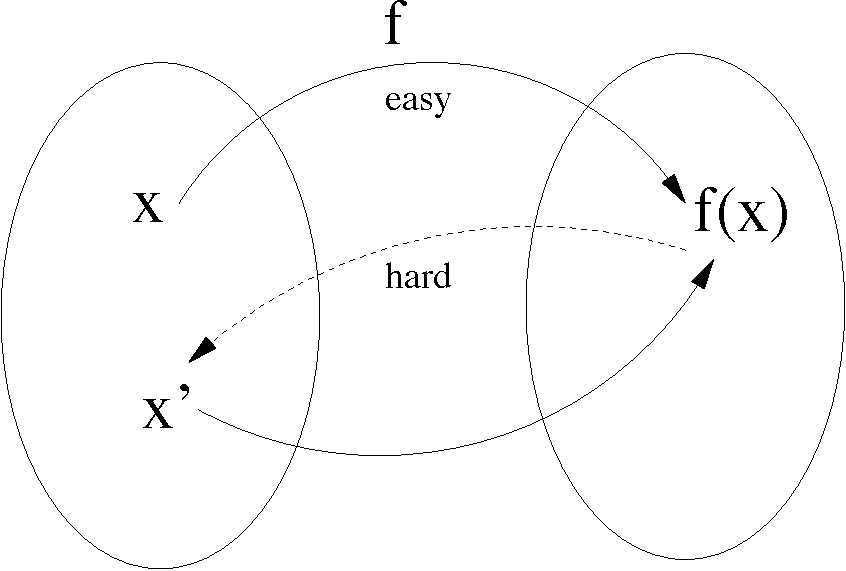
\includegraphics[width=4in]{fig1.pdf}

If you used a vector-graphics editor to create the image, send me also
the svg file (or whatever is the standard format for your program).

Use the predefined environments for theorems, lemmas, proofs, remarks, examples, 
and so on.

\end{document}
